%%
%% PhysioFlow -- SoftwareX manuscript (elsarticle, single column, OSP format)
%%

\documentclass[preprint,12pt,a4paper]{elsarticle}

\usepackage{amssymb}
\usepackage{hyperref}
\usepackage{graphicx}
\usepackage{booktabs}
\usepackage{url}
\usepackage{xurl}
\usepackage{tikz}
\usetikzlibrary{positioning, arrows.meta, shapes.geometric}
\usepackage{makecell}
\setlength{\parindent}{0pt}

\journal{SoftwareX}

\begin{document}
\renewcommand{\labelenumii}{\arabic{enumi}.\arabic{enumii}}

\begin{frontmatter}

\title{PhysioFlow: an open-source interactive platform for crop ecophysiology data analysis with statistical guard-rails}

\author[ifcat]{Daniel Hil\'ario da Silva}
\ead{daniel.hilario@ifgoiano.edu.br}

\author[ceagre,ifgr]{Leandro Rodrigues da Silva Souza\corref{cor1}}
\ead{leandrorodrigues.s@gmail.com}

\author[ifmt]{Andr\'e Abade}
\ead{andre.abade@ifmt.edu.br}

\author[ufmt]{Francisco de Almeida Lobo}
\ead{francisco.lobo@ufmt.br}

\author[ceagre,ifgr]{Fernando Rodrigues Cabral Filho}
\ead{fernandorcfilho10@gmail.com}

\author[ufrrj]{Erli Pinto dos Santos}
\ead{erli@ufrrj.br}

\author[ifgr]{Adinan Alves da Silva}
\ead{adinan.alves@ifgoiano.edu.br}

\author[ceagre]{Daiane Alves da Silva}
\ead{professoradaiane015@gmail.com}

\author[ifgr]{Ketlyn Santos Sousa}
\ead{ketlyn.s.sousa@gmail.com}

\author[ifgr]{Igor Eli da Silva}
\ead{igorelizoo@gmail.com}

\author[ifgr]{Alan Carlos da Costa}
\ead{alan.costa@ifgoiano.edu.br}

\address[ifcat]{Instituto Federal Goiano, Campus Catal\~ao, Goi\'as, Brazil}
\address[ceagre]{Center of Excellence in Exponential Agriculture (CEAGRE), Goi\'as, Brazil}
\address[ifgr]{Instituto Federal Goiano, Campus Rio Verde, Goi\'as, Brazil}
\address[ifmt]{Instituto Federal de Mato Grosso, Cuiab\'a, Mato Grosso, Brazil}
\address[ufmt]{Universidade Federal de Mato Grosso, Mato Grosso, Brazil}
\address[ufrrj]{Universidade Federal Rural do Rio de Janeiro, Serop\'edica, Rio de Janeiro, Brazil}

\cortext[cor1]{Corresponding author at: Center of Excellence in Exponential Agriculture (CEAGRE), Rio Verde, Goi\'as, Brazil.}

\begin{abstract}
Field ecophysiology campaigns based on infrared gas analyzers (IRGA), chlorophyll meters and ceptometers produce tabular datasets of gas-exchange, chlorophyll-fluorescence and leaf-area variables that must be cleaned, explored, modelled and mapped before publication. Instrument vendors provide no free open-source software for these stages, forcing researchers to write ad hoc scripts. We present \emph{PhysioFlow}, an open-source Python/Streamlit interactive platform that ingests CSV/XLSX exports, validates them against an explicit schema, and exposes a configurable replicate-handling pipeline, exploratory analysis with statistical guard-rails (categorical confounding via Cram\'er's V, VIF with derived-variable awareness, Kruskal--Wallis with minimum-N filtering, normality tests with companion Q--Q plots, multi-method outlier consensus), predictive modelling with optional GroupKFold, geospatial analysis in UTM metres and STL time-series decomposition with sparsity guard-rails, in a single code-free trilingual (PT/EN/ES) interface. Released under GPL-2.0 with a mandatory citation clause, it is used in the Goi\'as Verde initiative.
\end{abstract}

\begin{keyword}
Crop ecophysiology \sep Photosynthesis \sep IRGA \sep Exploratory data analysis \sep Statistical guard-rails \sep Reproducible research
\end{keyword}

\end{frontmatter}

%% ====================================================================
\section*{Required Metadata}

\section*{Current code version}

\begin{table}[!h]
\centering
\footnotesize
\begin{tabular}{|l|p{4.5cm}|p{6.5cm}|}
\hline
\textbf{Nr.} & \textbf{Code metadata description} & \textbf{Value} \\
\hline
C1 & Current code version & v1.0 \\
\hline
C2 & Permanent GitHub link to code/repository & \url{https://github.com/ML-Carbon-Project/physioFlow} \\
\hline
C3 & Legal Code License & GPLv2 with mandatory citation clause \\
\hline
C4 & Code versioning system used & git \\
\hline
C5 & Software code languages, tools, services used & Python 3.10+; Streamlit; pandas, NumPy, SciPy, scikit-learn, statsmodels; geopandas, shapely, pyproj, libpysal, esda; pytest \\
\hline
C6 & Compilation requirements, operating environments \& dependencies & Linux, macOS, Windows; Python $\geq 3.10$; \texttt{pip install -r requirements.txt} \\
\hline
C7 & Link to developer documentation/manual & \url{https://github.com/ML-Carbon-Project/physioFlow/tree/main/docs} \\
\hline
C8 & Support email for questions & \texttt{leandrorodrigues.s@gmail.com} \\
\hline
\end{tabular}
\caption{Code metadata (mandatory).}
\label{tbl:metadata}
\end{table}

%% ====================================================================
\section{Motivation and significance}\label{sec:intro}

Plant ecophysiology links the carbon, water and energy economy of crops to their environment, and its field measurement underpins decisions in agronomy, breeding and climate-change adaptation~\cite{Lambers2008,Long2006}. Three classes of portable instruments dominate field campaigns. Infrared gas analyzers (IRGA) housed in leaf chambers quantify net photosynthesis ($A$), transpiration ($E$), stomatal conductance ($g_s$) and internal/ambient CO$_2$ ($C_i$, $C_a$), from which derived efficiencies such as water-use efficiency (WUE), carboxylation efficiency ($A/C_i$) and the $C_i/C_a$ ratio are computed~\cite{Farquhar1980,vonCaemmerer2000,Long2003}. Chlorophyll fluorometers and chlorophyll-content meters report the effective quantum yield of photosystem~II ($Y_{II}$), the electron transport rate (ETR) and chlorophyll $a$/$b$~\cite{Maxwell2000,Baker2008}. Ceptometers estimate the leaf area index (LAI)~\cite{Breda2003}. Together they characterise the photosynthetic performance of a crop across genotypes, phenological stages, management systems and seasons. These measurements anchor agronomic studies of crop responses to irrigation and salinity, soil management and seasonal climate, in which leaf gas exchange and soil--plant carbon fluxes are read jointly to interpret productivity and stress~\cite{Oliveira2017,Munjonji2021,Peters2012,Sanchez2003,Guarrera2024}. In tropical agro-ecosystems such as the Brazilian Cerrado, where the present case study is set, characterising these fluxes is central both to yield management and to ecosystem carbon-balance accounting~\cite{Vourlitis2022}.

Each instrument exports a wide CSV/XLSX table in which a row is a leaf or canopy measurement carrying gas-exchange variables, fluorescence variables, chlorophyll and LAI replicates, plus metadata (crop, farm, land use, season, sampling point, coordinates, date). Turning this raw output into a publishable analysis still demands several non-trivial steps: standardising categorical fields; discarding rows without minimum agronomic information; consolidating field replicates of chlorophyll and LAI; running exploratory and inferential analyses; checking multicollinearity among the strongly derived physiological indices; inspecting the spatial structure of the campaign; decomposing temporal trends; and, optionally, fitting predictive models that relate measured traits to photosynthesis.

Despite the wide commercial availability of these instruments, manufacturers do not provide free, open-source software for the exploratory and modelling stages that transform raw exports into results. Vendor viewers focus on acquisition and quality control. Consequently, researchers must export the data and write custom scripts in R~\cite{Rcore} or Python, which poses a considerable barrier for agronomists, plant scientists and graduate students without formal training in programming or statistics. In most laboratories the intervening steps are still carried out manually or semi-automatically across spreadsheets and disconnected statistical packages, an approach that is time-consuming, error-prone, weakly standardised and hard to reproduce; in high-throughput campaigns this manual handling becomes an operational bottleneck that lowers analytical throughput and scientific productivity. The structure of ecophysiology field data also invites silent statistical errors: physiological indices are mutually derived (e.g.\ WUE $= A/E$), inflating multicollinearity by construction; sampling designs frequently alias farm, crop and land use, so an apparent ``between-farm'' difference may be an unidentifiable ``between-crop'' difference; replicated measurements at the same site induce pseudoreplication~\cite{Hurlbert1984} that inflates model skill; and short campaigns offer too few dates for meaningful seasonal decomposition.

Inspired by recent open-source efforts that bridged data analysis and end-users through a Streamlit interface~\cite{Streamlit}, and by our sibling platform for chamber-based soil greenhouse-gas flux analysis~\cite{DaSilva2026Goias}, we developed \emph{PhysioFlow} to consolidate the entire ecophysiology data-analysis workflow into a single configurable interactive platform. The distinguishing design choice is a set of \emph{statistical guard-rails} woven into the user interface: the application not only computes statistics but warns when their assumptions are violated. Recent original software publications in adjacent agronomic niches~\cite{Magnani2026apsimNGpy,Crecco2026prismatools} demonstrate the methodological value of releasing instrument-bound, end-to-end analytical pipelines as citable software, a precedent the present work follows for crop ecophysiology.

%% ====================================================================
\section{Software description}\label{sec:software}

\subsection{Software architecture}\label{sec:arch}

\emph{PhysioFlow} is implemented in Python~3.10~\cite{Streamlit,McKinney2010,Harris2020} and follows a \emph{session-state-centric, page-renderer pattern} typical of Streamlit applications, in which each page is a self-contained module that reads from and writes to a shared \texttt{st.session\_state} and consumes the cleaning, statistics and visualisation primitives in the \texttt{src/} package, so that costly I/O and cleaning operations happen at most once per session. The entry point \texttt{app.py} configures the page, checks whether Supabase authentication is enabled, and dispatches to the page renderer selected in the sidebar. Eight user-facing pages consume those primitives (Fig.~\ref{fig:architecture}).

\begin{figure}[!htb]
\centering
\resizebox{\linewidth}{!}{%
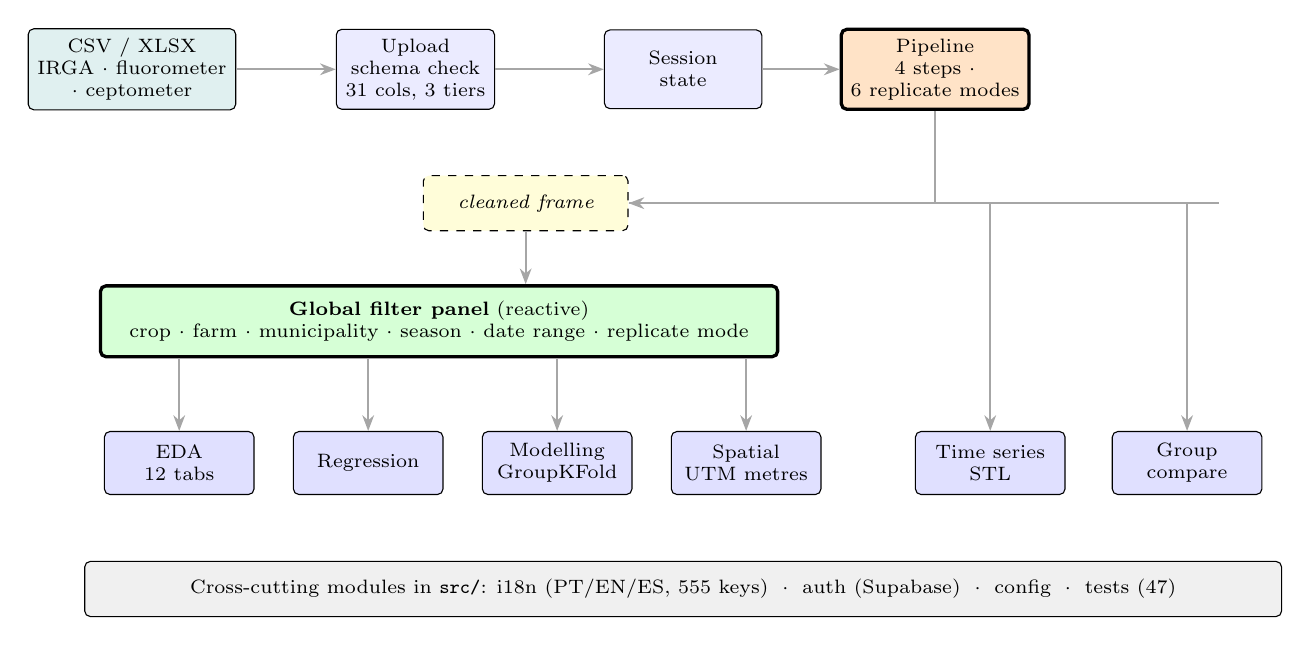
\begin{tikzpicture}[
  font=\scriptsize,
  src/.style={draw, rounded corners=2pt, minimum width=21mm, minimum height=10mm, fill=teal!12, align=center},
  proc/.style={draw, rounded corners=2pt, minimum width=20mm, minimum height=10mm, fill=blue!8, align=center},
  gate/.style={draw, rounded corners=2pt, minimum width=23mm, minimum height=10mm, fill=orange!22, align=center, very thick},
  frame/.style={draw, dashed, rounded corners=2pt, minimum width=26mm, minimum height=7mm, fill=yellow!15, align=center, font=\scriptsize\itshape},
  filt/.style={draw, rounded corners=2pt, minimum height=9mm, fill=green!16, align=center, very thick},
  page/.style={draw, rounded corners=2pt, minimum width=19mm, minimum height=8mm, fill=blue!12, align=center},
  band/.style={draw, rounded corners=2pt, minimum width=152mm, minimum height=7mm, fill=gray!12, align=center},
  arr/.style={->, >=Stealth, semithick, gray!70}
]
% --- ingestion row ---
\node[src]  (csv)      at (0,0)   {CSV / XLSX\\\scriptsize IRGA $\cdot$ fluorometer\\\scriptsize $\cdot$ ceptometer};
\node[proc] (upload)   at (3.6,0) {Upload\\\scriptsize schema check\\\scriptsize 31 cols, 3 tiers};
\node[proc] (state)    at (7.0,0) {Session\\state};
\node[gate] (pipeline) at (10.2,0){Pipeline\\\scriptsize 4 steps $\cdot$\\\scriptsize 6 replicate modes};
\draw[arr] (csv) -- (upload);
\draw[arr] (upload) -- (state);
\draw[arr] (state) -- (pipeline);

% --- cleaned frame ---
\node[frame] (cf) at (5.0,-1.7) {cleaned frame};
\draw[arr] (pipeline.south) |- (cf.east);

% --- global reactive filter (over the four analytical pages) ---
\node[filt, minimum width=86mm] (filter) at (3.9,-3.2)
  {\textbf{Global filter panel} (reactive)\\\scriptsize crop $\cdot$ farm $\cdot$ municipality $\cdot$ season $\cdot$ date range $\cdot$ replicate mode};
\draw[arr] (cf.south) -- (cf.south|-filter.north);

% --- analytical pages ---
\node[page] (eda)     at (0.6,-5.0) {EDA\\\scriptsize 12 tabs};
\node[page] (reg)     at (3.0,-5.0) {Regression};
\node[page] (model)   at (5.4,-5.0) {Modelling\\\scriptsize GroupKFold};
\node[page] (spatial) at (7.8,-5.0) {Spatial\\\scriptsize UTM metres};
\node[page] (ts)      at (10.9,-5.0){Time series\\\scriptsize STL};
\node[page] (cmp)     at (13.4,-5.0){Group\\compare};

\draw[arr] (eda.north|-filter.south)     -- (eda.north);
\draw[arr] (reg.north|-filter.south)     -- (reg.north);
\draw[arr] (model.north|-filter.south)   -- (model.north);
\draw[arr] (spatial.north|-filter.south) -- (spatial.north);
% time series and group comparison read the cleaned frame directly
\draw[semithick, gray!70] (cf.east) -- (13.8,-1.7);
\draw[arr] (10.9,-1.7) -- (ts.north);
\draw[arr] (13.4,-1.7) -- (cmp.north);

% --- cross-cutting band ---
\node[band] (cross) at (7.0,-6.6)
  {Cross-cutting modules in \texttt{src/}: i18n (PT/EN/ES, 555 keys) \;$\cdot$\; auth (Supabase) \;$\cdot$\; config \;$\cdot$\; tests (47)};
\end{tikzpicture}%
}
\caption{High-level data-flow architecture of \emph{PhysioFlow}. Raw exports from IRGA, chlorophyll-fluorometer and ceptometer instruments are validated against the reference schema at upload, cached in the Streamlit session state, and consumed by the Pipeline, which produces a single cleaned frame. A shared, reactive \emph{global filter panel} (crop, farm, municipality, season, date range and replicate mode) is injected at the top of the four analytical pages (EDA, Regression, Modelling, Spatial) and propagates instantly to every chart, test and model; the Time Series and Group-comparison pages read the cleaned frame directly through their own controls. Library stack: Pipeline $\to$ \texttt{pandas}/\texttt{NumPy}; modelling $\to$ \texttt{scikit-learn}~\cite{Pedregosa2011}; inference $\to$ \texttt{SciPy}/\texttt{statsmodels}; visualisation $\to$ \texttt{seaborn}~\cite{Waskom2021,Hunter2007}; geospatial $\to$ \texttt{geopandas}, \texttt{pyproj}, \texttt{libpysal}/\texttt{esda}~\cite{Rey2010Pysal}.}\label{fig:architecture}
\end{figure}

The \texttt{src/} package is organised by concern. \texttt{schema.py} declares a reference dictionary of 31 columns in three severity tiers (required, recommended, optional), each mapped to the dependent feature, and validates types and coordinate ranges without blocking the upload. \texttt{pipeline.py} hosts the deterministic cleaning primitives and a robust date-column detector that coerces heterogeneous Excel \texttt{object} columns to \texttt{datetime64}. \texttt{stats\_utils.py} implements bias-corrected Cram\'er's V~\cite{Bergsma2013} and a categorical-confounding auditor. \texttt{ml/model\_registry.py} registers five supervised regression estimators (Linear Regression, Ridge, Random Forest~\cite{Breiman2001}, Gradient Boosting~\cite{Friedman2001}, $k$-NN) wrapped in a \texttt{scikit-learn} pipeline. Cross-cutting modules under \texttt{i18n/} (555 keys at full PT/EN/ES parity), \texttt{auth/}, \texttt{config/} and \texttt{tests/} (47 \texttt{pytest} functions) serve every page.

The implementation follows established software-engineering practices: public functions in \texttt{src/} carry type annotations; the suite covers 86\% of the schema validator and 89\% of the confounding utilities (measured with \texttt{pytest --cov}); \texttt{ruff} enforces style and \texttt{mypy} validates static types on the analytical core; and a GitHub Actions workflow runs the test, lint and type-check matrix on Python 3.10--3.12 for every push and pull request. New estimators, cleaning primitives and schema columns are added declaratively through the corresponding registries in \texttt{src/}, so the user interface extends itself without bespoke widget code.

\subsection{Software functionalities}\label{sec:functions}

\paragraph{Upload (Fig.~\ref{fig:upload}).} Accepts CSV, XLSX and XLS files. After parsing, the schema validator classifies every expected column as \emph{required}, \emph{recommended} or \emph{optional}, checks data types, flags columns that exist but are 100\% empty (distinct from ``missing''), and verifies that latitude/longitude lie within plausible ranges. Missing columns disable dependent features without blocking the upload.

\begin{figure}[!htb]
  \centering
  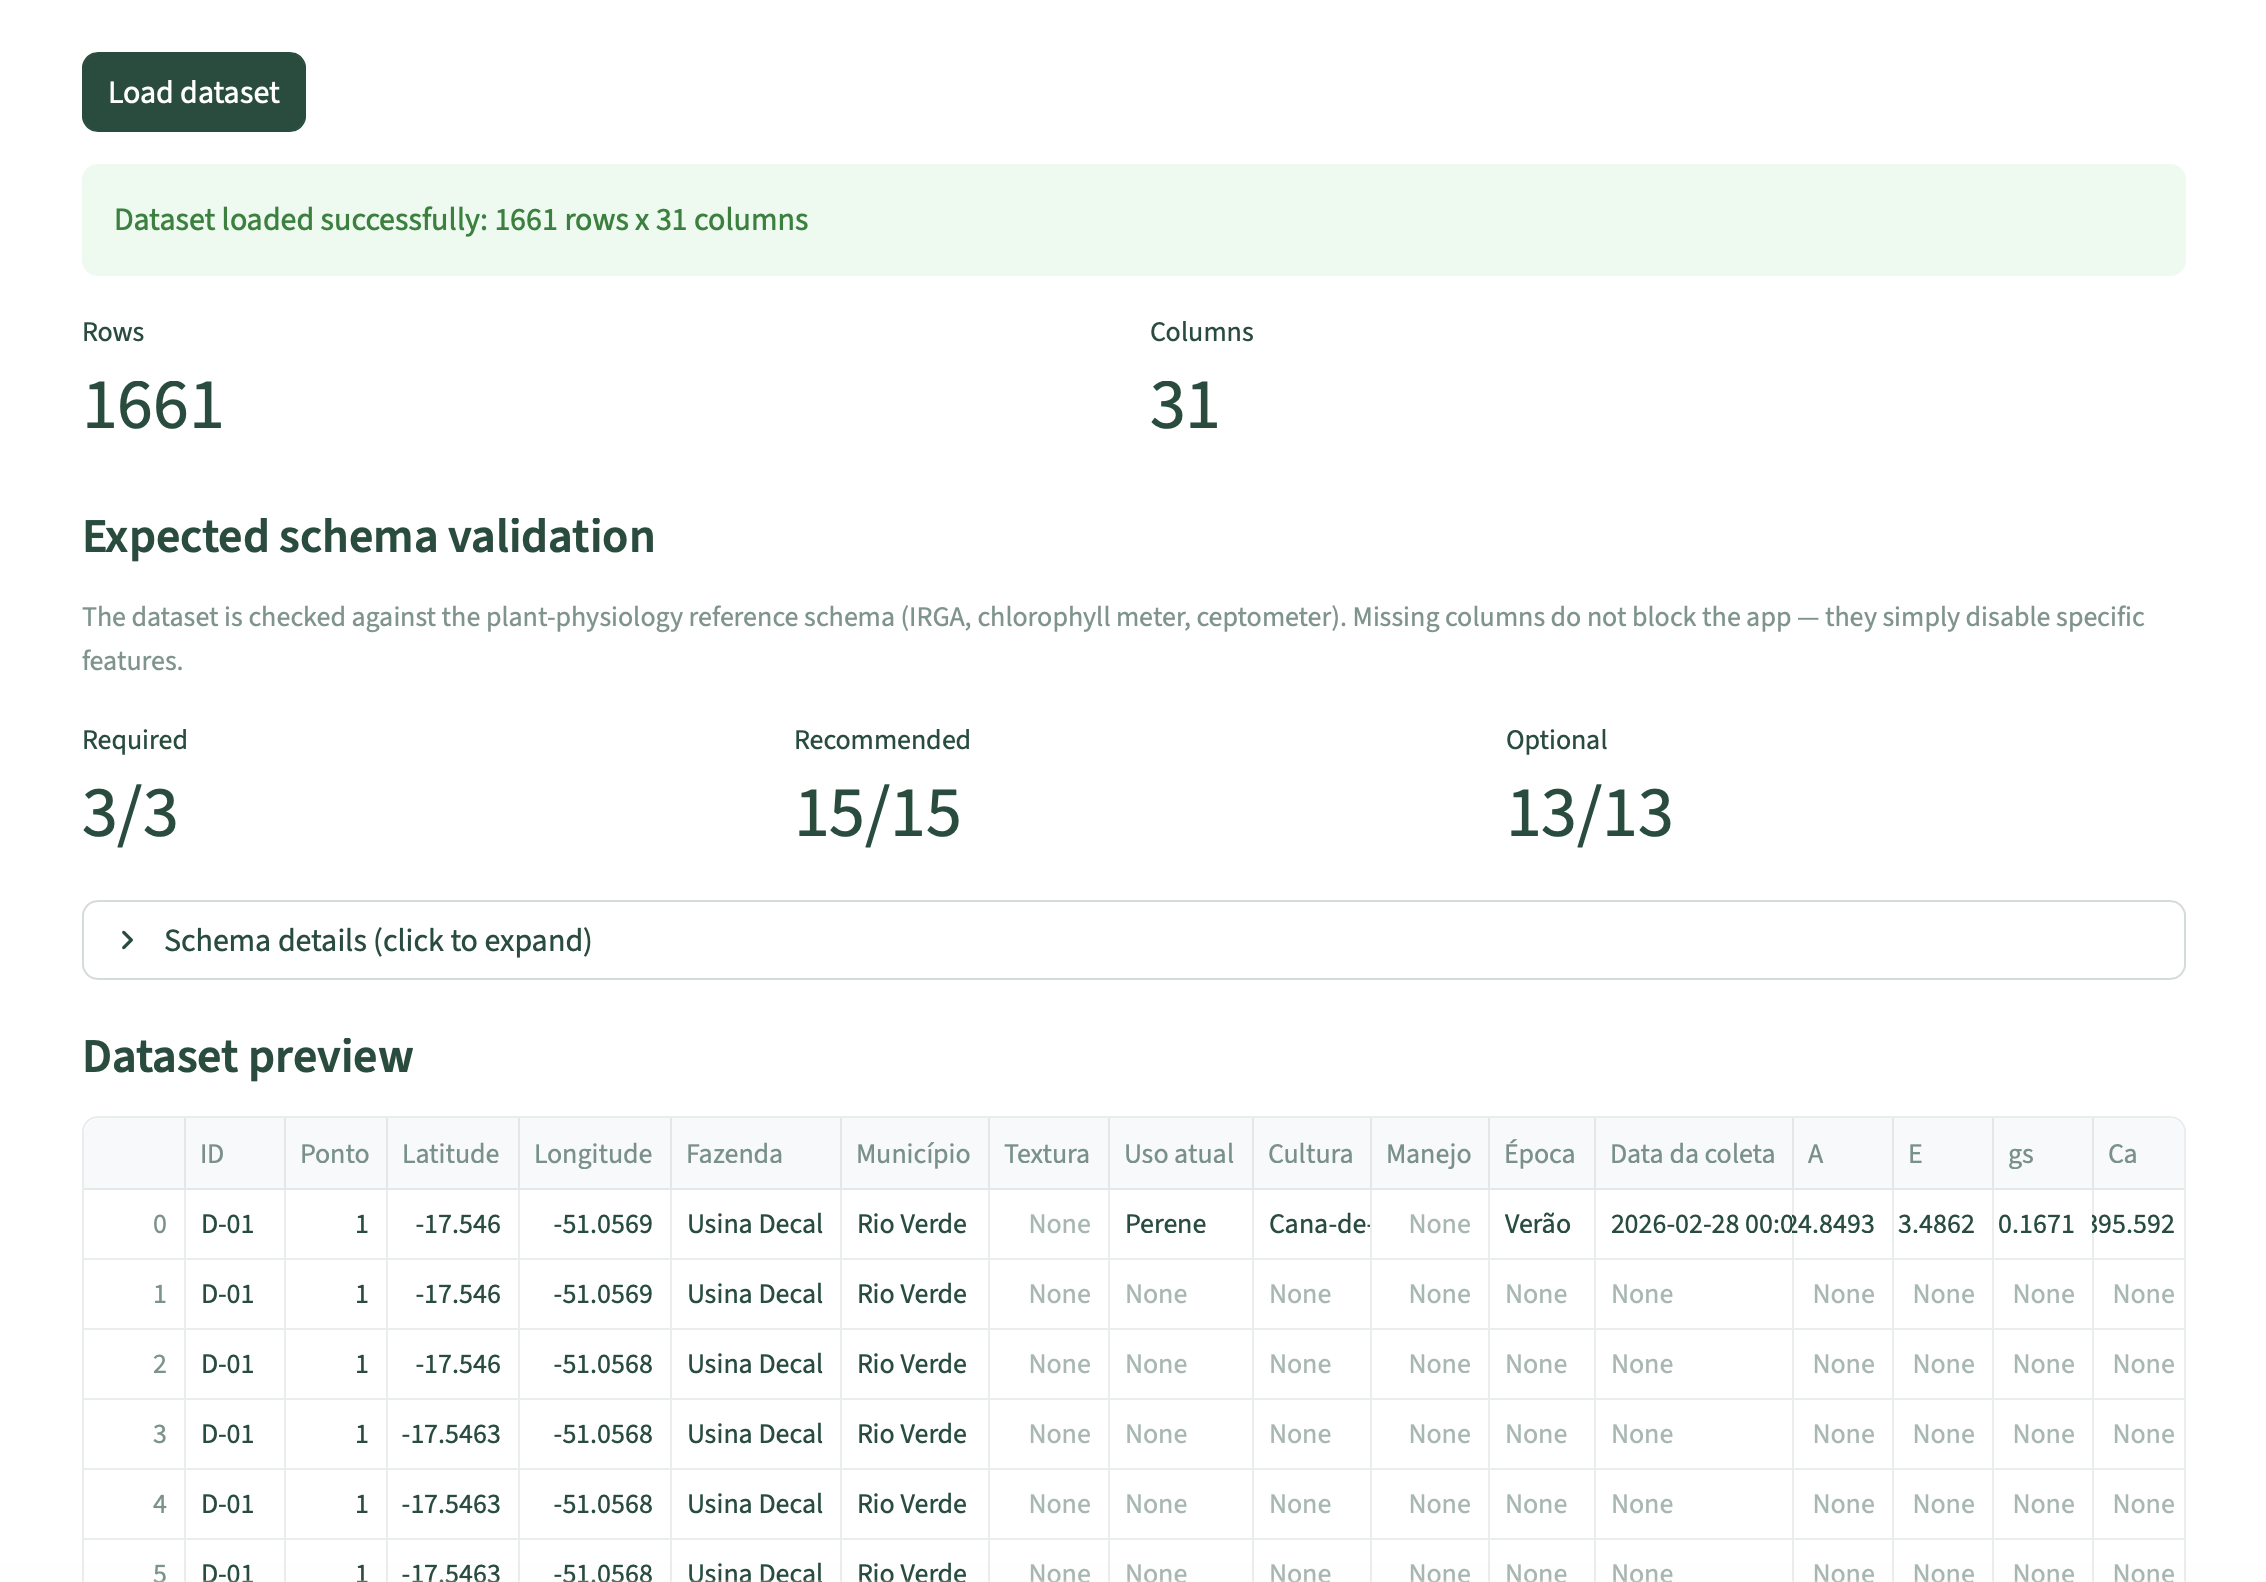
\includegraphics[width=\linewidth]{figs/upload_schema.png}
  \caption{Upload page after ingestion of an ecophysiology dataset. The schema validator reports each expected column with its severity tier, the resolved column name, the detected type and the dependent feature.}\label{fig:upload}
\end{figure}

\paragraph{Pipeline.} Four deterministic steps --- text standardisation, removal of rows without essential metadata, removal of empty grid points, and replicate treatment --- followed by a tabular step-by-step report (Fig.~\ref{fig:pipeline}) recording rows in/out and percentage removed at each step, with a warning whenever any step discards more than 50\% of the rows. Replicates of chlorophyll and LAI can be handled in six modes: mean, \emph{median} (robust to outliers; added at the suggestion of an external researcher), replicate-unfolding into independent rows, and exclusive selection of replicate~1, 2 or~3.

\begin{figure}[!htb]
  \centering
  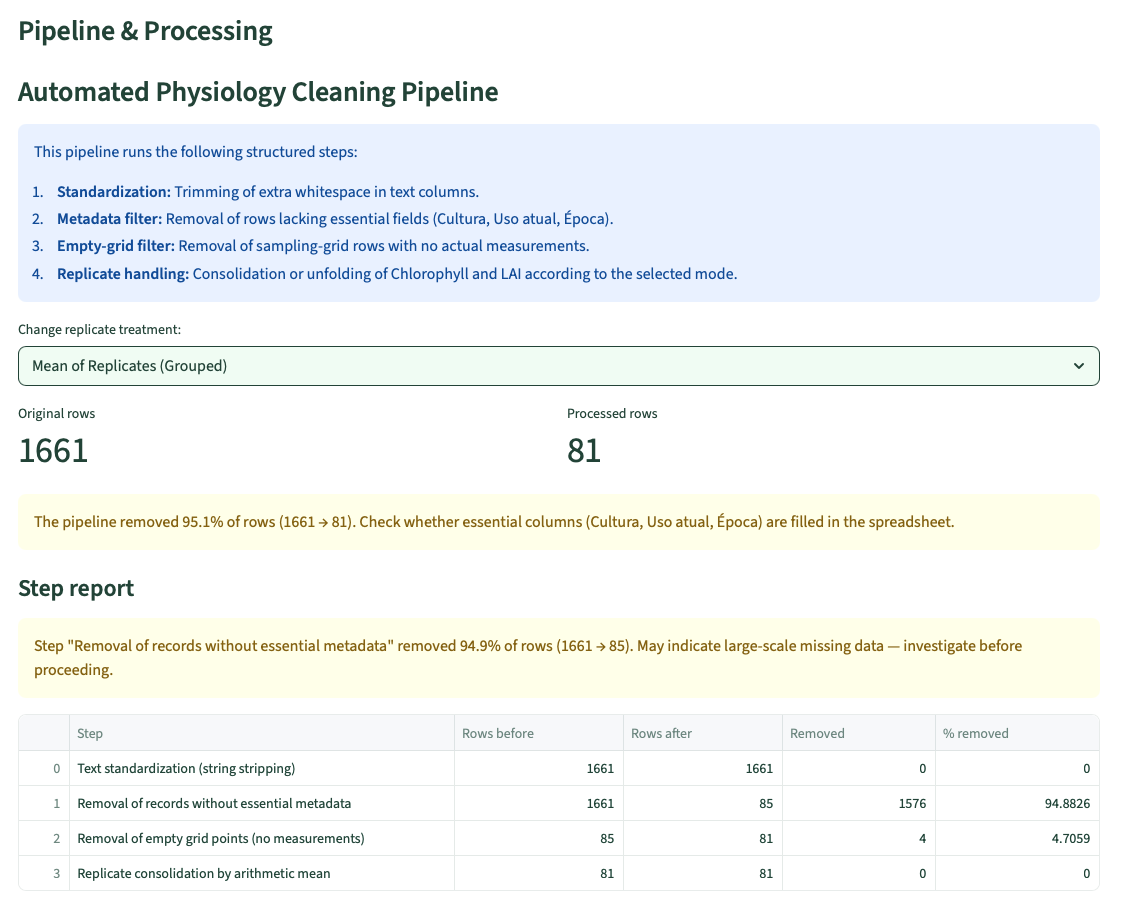
\includegraphics[width=\linewidth]{figs/pipeline_audit.png}
  \caption{Step-by-step audit of the cleaning pipeline applied to the real Rio Verde dataset. Each row reports lines before/after and the share removed; the essential-metadata filter alone removes 94.9\% of the raw rows, triggering the high-discard warning.}\label{fig:pipeline}
\end{figure}

\paragraph{Exploratory Data Analysis.} Twelve tabs: descriptive statistics; a data-quality tab that audits categorical \emph{confounding} via Cram\'er's V (Fig.~\ref{fig:confounding}); univariate distributions with KDE; boxplots by group; pair plots; Pearson, Spearman or Kendall correlation matrices; a lat/lon scatter map; temporal aggregation; categorical composition charts; non-parametric inference (Kruskal--Wallis~\cite{Kruskal1952} with a minimum-N-per-group slider, Shapiro--Wilk~\cite{ShapiroWilk1965} accompanied by Q--Q plots, and VIF~\cite{Belsley1980VIF} with an explicit caveat that derived indices such as $C_i/C_a$, $A/C_i$ and WUE inflate VIF by construction); a top-$N$ hotspots ranking; and a multi-method outlier audit (Z-score, IQR, Isolation Forest~\cite{Liu2008}, Local Outlier Factor~\cite{Breunig2000}, Elliptic Envelope) with a consensus criterion and an assumptions caption.

\begin{figure}[!htb]
  \centering
  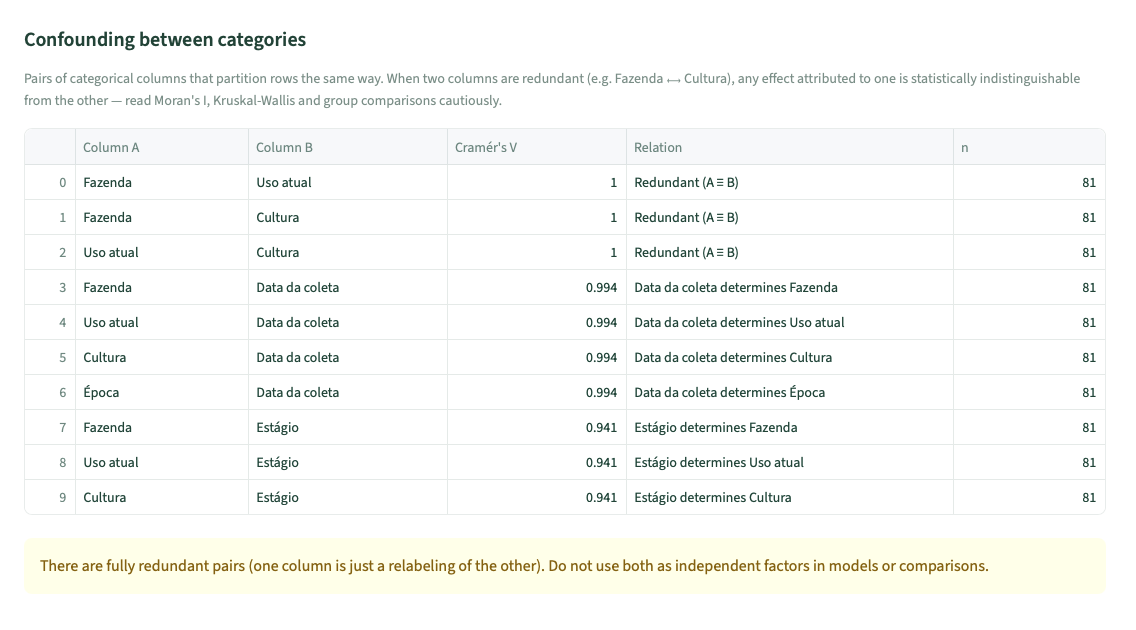
\includegraphics[width=\linewidth]{figs/confounding.png}
  \caption{Data-quality tab auditing categorical confounding. On the Rio Verde dataset the tool detects that \emph{Fazenda} (farm), \emph{Cultura} (crop) and \emph{Uso atual} (land use) are perfectly redundant (Cram\'er's V $=1.00$), warning the user that between-group contrasts on these fields are statistically unidentifiable.}\label{fig:confounding}
\end{figure}

\paragraph{Regression and Modelling.} The Regression page offers physiological bivariate presets (e.g.\ $g_s$ vs.\ $A$, $C_i$ vs.\ $A$) and free custom regression. The Modelling page registers five estimators and reports holdout $R^2$, MAE, RMSE and cross-validated $R^2$, with an \emph{optional GroupKFold} and a grouping-column selector (default a synthetic \emph{farm + point} key) to mitigate pseudoreplication~\cite{Hurlbert1984}.

\paragraph{Spatial Analysis.} IDW interpolation, global Moran's I and LISA cluster maps~\cite{Anselin1995}, Getis--Ord $G_i^*$~\cite{Getis1992}, UTM grid aggregation, ordinary kriging~\cite{Cressie1993} with a fitted spherical variogram, and an optional municipality basemap. All distance-based computations are performed in \emph{UTM metres} with an EPSG code derived automatically from the mean longitude, correcting the anisotropy of degree-based latitude/longitude distances.

\paragraph{Time Series.} Daily resampling (mean or median) and STL decomposition~\cite{Cleveland1990STL}, \emph{blocked when fewer than ten distinct dates are present} so that sparse campaigns do not yield a decomposition dominated by interpolation.

\paragraph{Two-group comparison and Authentication.} A comparative page partitions the dataset via manual multi-select or a case-insensitive substring pattern and returns a Mann--Whitney U test~\cite{Mann1947} per variable, paired log-linear regressions and an hourly profile. An optional Supabase login (disabled by default) adds email/password authentication; the application is fully functional without configuration.

%% ====================================================================
\section{Illustrative example}\label{sec:examples}

A real ecophysiology campaign in Rio Verde, GO (Brazilian Cerrado), comprising 1\,661 raw measurement rows across soybean and sugarcane fields, was ingested via the Upload page. The schema validator confirmed the required metadata and physiological variables and flagged the \emph{Manejo} (soil management) and \emph{Textura} (soil texture) columns as present but 100\% empty.

The Pipeline was run with the default mean replicate mode. Its audit trail (Fig.~\ref{fig:pipeline}) traces 1\,661 input rows down to 81 sampling-point records: the essential-metadata filter alone removes 94.9\% of the raw rows --- an incomplete sampling grid in which most planned points carry no measurement --- triggering the high-discard warning that alerts the user before any inference is attempted.

The cleaned frame was then submitted to the EDA data-quality tab (Fig.~\ref{fig:confounding}). The Cram\'er's V auditor reported that \emph{Fazenda}, \emph{Cultura} and \emph{Uso atual} are mutually redundant (Cram\'er's V $=1.00$): the two surviving farms map one-to-one onto the two crops (Usina Decal $\equiv$ sugarcane, 27 records; Reunidas Baumgart $\equiv$ soybean, 54 records). The guard-rail makes explicit that any nominally ``between-farm'' contrast is an unidentifiable ``between-crop'' contrast --- a confounding that a naive grouped comparison or a high spatial autocorrelation statistic would silently misattribute to spatial structure.

The Modelling page then predicted net photosynthesis ($A$, $n=71$) from gas-exchange, fluorescence and chlorophyll predictors, comparing five supervised regressors in a single run under GroupKFold cross-validation keyed on the synthetic \emph{farm + point} group to curb pseudoreplication (Fig.~\ref{fig:modeling}); Linear Regression attained the highest cross-validated skill (CV $R^2 = 0.95$), with the tree ensembles close behind. Finally, the Time Series page was invoked: with only three distinct collection dates (2025-12-19 to 2026-02-28), the STL guard-rail \emph{blocked} the decomposition and explained why (Fig.~\ref{fig:stl}), rather than returning a seasonal component that would be 90\% interpolation.

\begin{figure}[!htb]
  \centering
  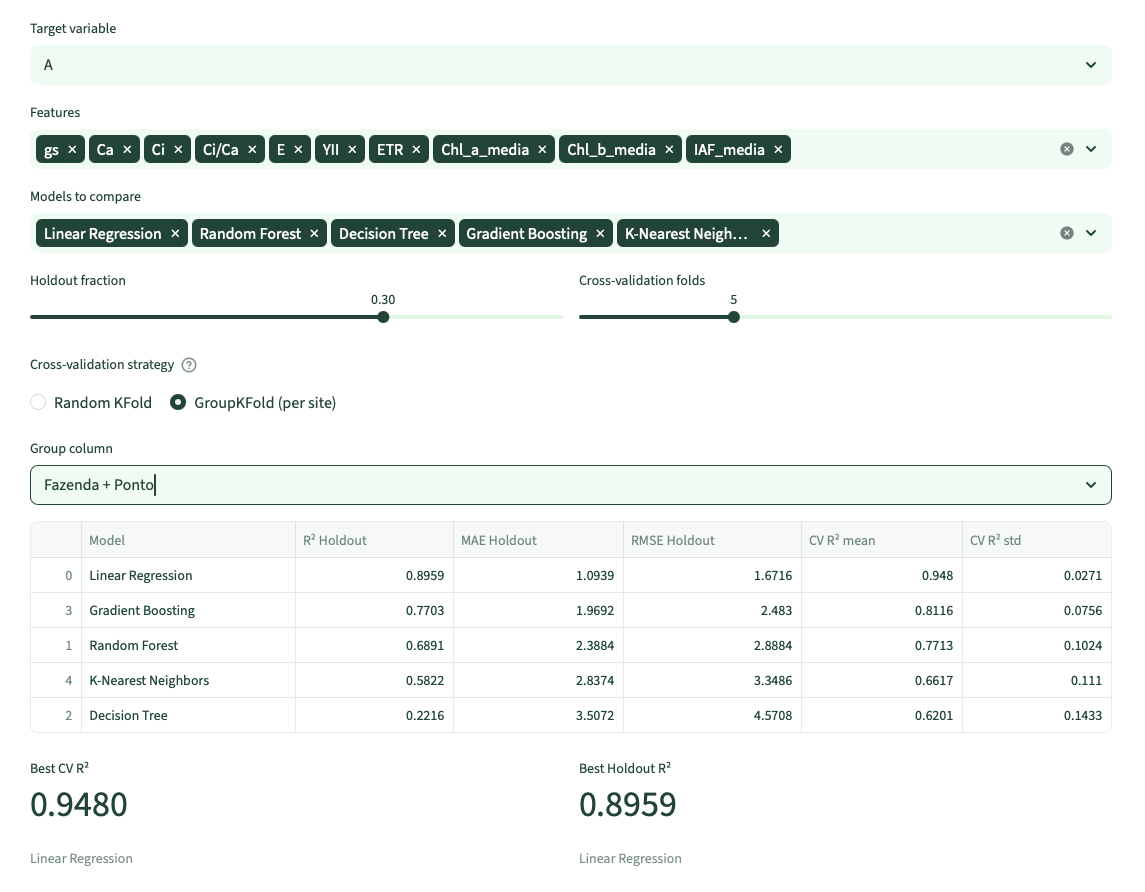
\includegraphics[width=\linewidth]{figs/modeling_comparison.png}
  \caption{Modelling page comparing five supervised regressors for net photosynthesis ($A$) on the Rio Verde dataset in a single run, reporting holdout $R^2$, MAE and RMSE alongside cross-validated $R^2$ (mean and standard deviation). Linear Regression attains the highest cross-validated skill, with the tree ensembles close behind; here the GroupKFold-per-site guard-rail (grouping on \emph{farm + point}) is enabled to curb pseudoreplication.}\label{fig:modeling}
\end{figure}

\begin{figure}[!htb]
  \centering
  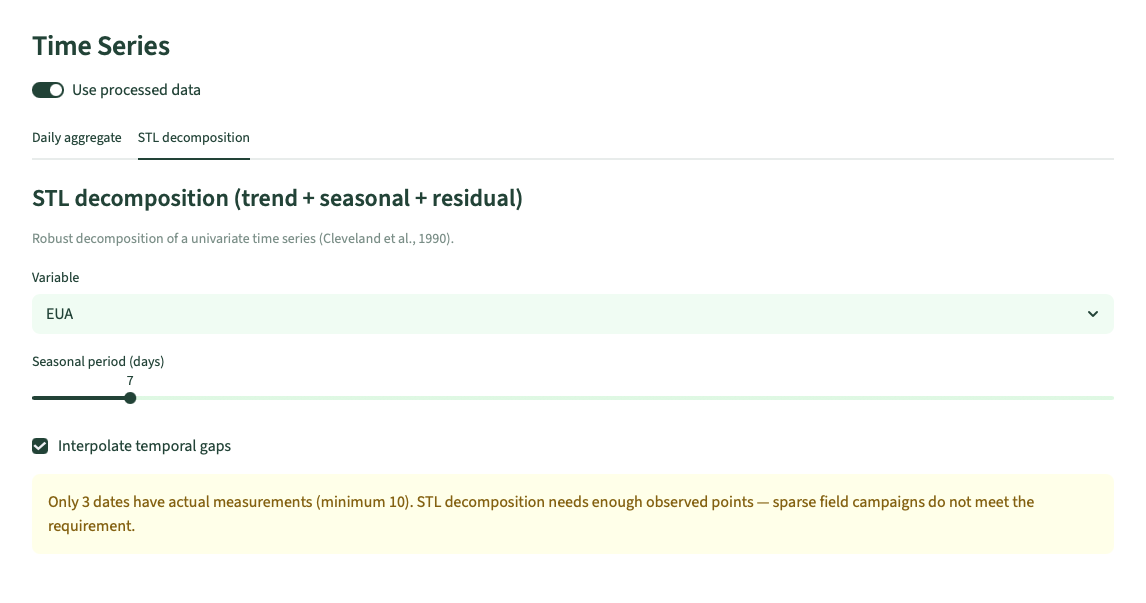
\includegraphics[width=\linewidth]{figs/stl_blocked.png}
  \caption{Time Series page on the Rio Verde dataset. Because the campaign contains only three distinct collection dates, below the ten-date threshold, the STL guard-rail blocks the decomposition and reports the reason instead of producing an interpolation-dominated result.}\label{fig:stl}
\end{figure}

End-to-end, the four-step pipeline on the 1\,661-row dataset completes in under two seconds on a 16\,GB-RAM laptop (Python~3.10, pandas~2.0), and each EDA tab, model fit and spatial computation renders interactively without leaving the browser.

%% ====================================================================
\section{Impact}\label{sec:impact}

PhysioFlow brings the cleaning, exploratory analysis and supervised modelling needed to interpret crop-ecophysiology data into a single interactive platform, closing a gap left by instrument manufacturers, who provide no free or open-source tools for these stages. For agronomists, plant scientists and graduate students without a programming background, especially in developing countries and under-resourced institutions, this barrier often postpones the analysis of field campaigns that already demand considerable investment in equipment, logistics and labour.

PhysioFlow's main contribution is methodological, not just operational: its statistical guard-rails turn assumptions that researchers usually check informally, or skip, into explicit on-screen warnings. The Cram\'er's V confounding auditor, the VIF caveat for derived physiological indices, the minimum-N filter for Kruskal--Wallis, the Q--Q plots beside normality tests, the optional GroupKFold against pseudoreplication, and the sparsity block on STL collectively steer non-statistician users away from these failure modes. In the Rio Verde campaign these guard-rails immediately surfaced a perfectly confounded design and a campaign too short for seasonal decomposition, diagnostics that might otherwise have surfaced, if at all, only at peer review.

\emph{PhysioFlow} is currently used within the Goi\'as Verde initiative (Instituto Federal Goiano and CEAGRE) to analyse the photosynthetic performance of soybean and sugarcane across cropping systems of the Brazilian Cerrado, and it supports the data-analysis training of several graduate students and their supervisees in the associated post-graduate programme, who use the application both for their own datasets and for teaching. An earlier sibling of the platform, targeting soil greenhouse-gas fluxes, was published and presented to the agronomy and remote-sensing community at the 1st International Symposium on Climate and Agricultural Resilience / 5th CEAGRE Agro Experience, where its four core analytical modules were also delivered as a hands-on training workshop~\cite{DaSilva2026Goias}. Because it is open-source, free of licensing fees and dataset-agnostic, the tool is reusable for any tabular research dataset that requires diagnostic-driven cleaning, EDA and supervised regression, with adjacent potential in digital agriculture, high-throughput plant phenotyping, environmental monitoring and climate-change research; its trilingual (PT/EN/ES) interface broadens reach across the Ibero-American research community. The current release (v1.0) comprises approximately 4{,}800 lines of Python across the \texttt{src/} package, 47 \texttt{pytest} unit tests and 555 user-interface keys at full PT/EN/ES parity. Preliminary feedback from collaborating laboratories suggests a reduction in analysis time from several days of manual spreadsheet operations and ad hoc scripts to a few hours within the interactive interface, letting researchers spend their time on the biological interpretation of the results rather than on repetitive data manipulation.

%% ====================================================================
\section{Conclusions}\label{sec:conclusions}

We presented \emph{PhysioFlow}, an open-source Python/Streamlit interactive platform for crop-ecophysiology datasets produced by IRGA, chlorophyll-meter and ceptometer instruments. The platform consolidates ingestion, schema validation, a configurable six-mode replicate pipeline, exploratory analysis with statistical guard-rails, multi-method outlier auditing, bivariate and machine-learning regression with optional GroupKFold, geospatial analysis in UTM metres (IDW, Moran's I/LISA, Getis--Ord $G_i^*$, ordinary kriging) and STL time-series decomposition with a sparsity block, into a single trilingual interface.

Its distinguishing feature is the integration of contextual statistical guard-rails directly into the user interface, helping non-statistician users avoid the confounding, multicollinearity, pseudoreplication and sparsity pitfalls common in ecophysiology field data, as demonstrated on a real Cerrado campaign.

Planned developments include physiological range validation in the schema (\texttt{valid\_range} per column), integration of the instrument data dictionary as in-app tooltips, raising test coverage above 70\% across the \texttt{ml/}, \texttt{state} and \texttt{auth} modules, a quasi-constant-variable warning in the correlation panel, and a public Docker image for one-command deployment. On the analytical side, automatic fitting of physiological response curves (e.g.\ $A$/$C_i$ and light-response curves), automated report export, and predictive guard-rails that flag physiological-stress patterns to support decision-making are planned as future directions.

%% ====================================================================
\section*{Acknowledgements}

The authors thank the Ministry of Science, Technology and Innovation (MCTI), the Brazilian Funding Authority for Studies and Projects (FINEP), the Goi\'as State Research Foundation (FAPEG), the National Council for Scientific and Technological Development (CNPq), the Coordination for the Improvement of Higher Education Personnel (CAPES), the State Secretariat for Development and Innovation of Goi\'as (SECTI), the Center of Excellence in Exponential Agriculture (CEAGRE), and the Instituto Federal Goiano for supporting the research developed.

%% ====================================================================
\bibliographystyle{elsarticle-num}
\bibliography{refs}

\end{document}
